\section{Värmeutveckling}

\textbf{
HAREC a.\ref{HAREC.a.2.7}\label{myHAREC.a.2.7}
}

\index{värmeutveckling}
\index{heat dissipation}

\subsection{Värmeledning}

\textbf{
HAREC a.\ref{HAREC.a.2.7.1}\label{myHAREC.a.2.7.1}
}

\index{värmeledning}
\index{heat transfer}
\index{termisk resistans}
\index{symbol!\(R_\Theta\) termisk resistans}
\index{ambient temperature}
\index{symbol!\(T_A\) ambient temperature}
\index{elsäkerhet}
\index{kalllödning}

Vi har tidigare betraktat Joules lag för effektutveckling i motstånd.
Det är dags att börja utveckla en lite mer komplett syn på värmeutveckling.
Ett motstånd som utvecklar 1~Watt kommer stiga i temperatur tills dess att
jämvikt uppstår mellan motståndets förmåga att avleda värme och
omgivningstemperaturen.

\emph{Termisk resistans} (eng. \emph{thermal resistance}) är ett mått på
hur bra ett material är på att leda värme och har symbolen \(R_\Theta\),
och anges i enheten kelvin per Watt. Temperaturen \(T_k\) för en
komponent beror på medeleffekten \(P\) den producerar i värme, den
termiska resistansen samt \emph{omgivande temperatur} (eng.
\emph{ambient temperature}) \(T_A\) enligt:

\(T_k = T_A + R_\Theta \cdot P\)

Den termiska resistansen för komponent, kylpasta, isolerskiva och kylfläns
kan summeras precis som resistansen för vanliga motstånd och det
sammanlagda värdet används sedan för att beräkna temperaturen på en
komponent eller behovet av kylfläns.

\subsection{Konvektion}
\textbf{
HAREC a.\ref{HAREC.a.2.7.2}\label{myHAREC.a.2.7.2}
}
\index{konvektion}
\index{kylfläns}
\index{heatpipe}

\emph{Konvektion} (eng. \emph{convection}) är när värme skapar ett
naturligt flöde i vätska eller gas, oftast luft. När luft värms upp så
vill den expandera, varvid densiteten sjunker och luften vill stiga uppåt.
Kallare luft strömmar då till och kan därmed kyla värmekällan. En stor
temperaturskillnad medför att konvektionen ökar och därmed en bättre
kylning.

För t.ex. transistorer kan värmealstringen ske på en sådan liten yta att
konvektion från komponenten inte räcker för att kyla bort den producerade
värmen. Därför monterar man dem på en \emph{kylfläns} (eng.
\emph{heat sink}) som fördelar värmen över en större yta så att verkan av
konvektion ökar.

En effektiv metod att transportera värme är via en så kallad \emph{heat pipe}.
Det är ett rör innehållande en vätska som förångas vid en temperatur strax över
rumstemperatur och då effektivt leder överskottsvärme till ett plats där den kan
kylas bort. Heat pipe används numera ofta i datorer och solfångare.

Om värme produceras på en lite yta kan man behöva hjälpa konvektionen, vilket
ibland kallas för \emph{forcerad konvektion} (eng. \emph{forced convection}).
Med hjälp av fläkt blåses luft mot eller sugs förbi kylflänsen vilket ökar
värmeutbytet. Eftersom fläktar skapar oljud brukar man försöka anpassa
fläktens varvtal i förhållande till temperaturen, men även en variation av
varvtal kan uppfattas som störande. Andra åtgärder för att minska ljudnivån
är att skapa släta ytor för luften så det inte bildas luftvirvlar eller
styra in och utgående luftflödet med bafflar.

Ett problem som kan uppstå är att utrustning som är gjord för självkonvektion
blir placerad eller monterad så att luftkylning inte kan flöda fritt runt
utrustningen. Detta kan leda till överhettning på motsvarande sätt som när
en fläkt för forcerad kylning går sönder. Dålig termisk kontakt mellan
transistor och kylfläns är ett annat exempel på hur dålig värmeledning skapar
problem med överhettning.

\subsection{Värmealstring}
\textbf{
HAREC a.\ref{HAREC.a.2.7.4}\label{myHAREC.a.2.7.4}
}
\index{värmealstring}

\emph{Värmealstring} kan ske på fler ställen än motstånd. Lite förenklat
kan man säga att alla komponenter har förluster som producerar värme. Genom
lämpligt val av komponenter och korrekt dimensionering kan vi undvika att
producera onödiga värmeförluster. Kraftaggregat och effektsteg är exempel
på apparater där det går större strömmar vilka ofrånkomligen också alstrar
mera värme. Lägre förluster skapar man genom att helt enkelt ha bättre
ledningsförmåga, lägre resistans. Det är dock för många delar av designen
högst försumbara förluster som inte kräver någon större hänsyn för att få
det att överleva.

Även halvledare skapar värme, och även här gäller Joules lag med spänning
gånger ström. I ett effektsteg t.ex. så kommer transistorn ''bränna'' av
effekten för spänningen över transistorn gånger strömmen genom den. Onödigt
hög spänning och ström skapar högre värmeutveckling, vilket är en anledning
till att man gärna undviker slutsteg som arbetar i klass A till fördel för
slutsteg som arbetar i klass AB, B eller C.

Bristande värmeavledning leder ofta till ett katastrofalt fel, som t.ex.
sönderbrända motstånd och transistorer. Även ledare kan brinna av när man
har för liten ledararea, och därmed för hög resistans, för den ström som
ska gå genom den. Av det skälet finns det dimensioneringsregler t.ex.
krav på minsta arean av koppar i ledare helt enkelt för att de inte ska
skapa brand.

En annan effekt av värmeledning är att det kan ibland vara svårt att löda
på kretskort, framför allt vid ledare som går mot stora kopparytor som
har en relativt god värmeledningsförmåga. Ibland designar man små mönster
''thermals'' runt sådana lödpunkter för att minska värmeavledningen.
Ett effektivt sätt att kunna löda och framförallt löda av från sådana
kort är att man förvärmer hela kretskortet eller området runt om
lödpunkten. Då kommer temperaturskillnaden mellan lödpennans spets och
omgivningen att minska och då krävs det inte lika stor effekt för att få
upp lödpunkten i rätt temperatur för att kunna genomföra lödningen med god
\emph{vätning} och därmed undvika att det bildas en ''kallödning''.

\subsection{Värme i transistor}
\textbf{
HAREC a.\ref{HAREC.a.2.7.3}\label{myHAREC.a.2.7.3}
}

För att förstå värmealstring i en transistor så börjar vi med att tänka oss
att vi har en transistor som matas med 12~V matspänning. Vi genererar då en
10~Vpp (topp-topp-spänning) sinus in i en last med 50~Ohm. Vad är effekt-
förlusten i transistorn?

\begin{figure}[h]
\begin{center}
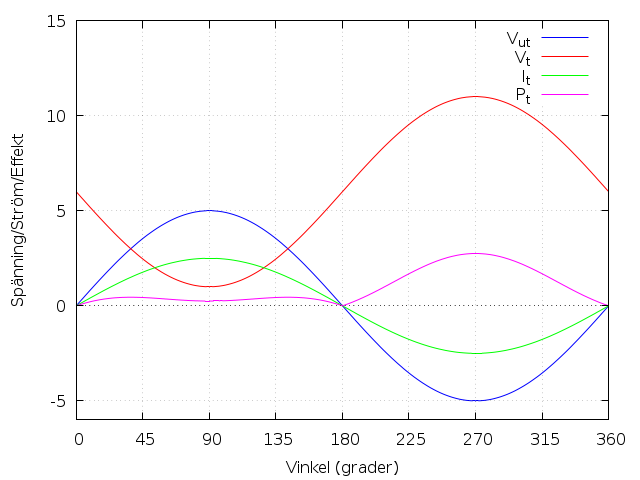
\includegraphics[width=7cm]{images/power1.png}
\caption{Utspänning $V_{ut}$, Transistor-spänning $V_t$, Transistor-ström $I_t$ och transistor-effekt $P_t$ varierar med vinkel sinus-signalen för resistiv last.}
\label{fig:power1}
\end{center}
\end{figure}

I bild \ref{fig:power1} ser vi utsignalen \(V_ut\) som en sinus med amplituden
\(5\ V\), dvs \(10\ V_{pp}\). Eftersom transistor har en vilo-spänning på 6~V
för att få marginal mot \(0\ V\) och \(+12\ V\), så kommer spänningen variera
mellan \(1\ V\) och \(11\ V\) och det ser man i \(V_t\) kurvan. Utgångslastens
resistor lastar med en ström \(I_t\) som är proportionerlig mot spänningen
\(V_{ut}\) på utgången. Effekten för transistorn \(P_t\) är sedan absolut-
funktionen för strömmen gånger spänningen, dvs. Joules lag. Den observante ser
att effekten är signifikant högre för andra halvan av kurvan, då man har både
hög spänning och hög ström.
